\documentclass[tikz,border=10pt]{standalone}
\usetikzlibrary{calc}
\begin{document}
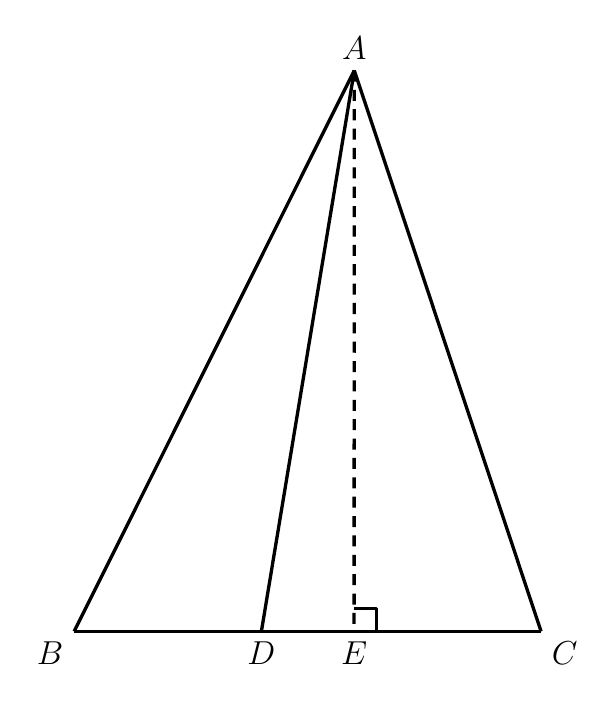
\begin{tikzpicture}[line width=1.2pt, line join=round]
\coordinate (A) at (0.584,3.568);
\coordinate (B) at (-2.974,-3.555);
\coordinate (C) at (2.956,-3.555);
\coordinate (D) at (-0.596,-3.555);



\coordinate (E) at (0.581,-3.555);


\draw (A) -- (B);
\draw (A) -- (C);
\draw (A) -- (D);


\draw (B) -- (D) -- (E) -- (C);


\draw[dash pattern=on 4pt off 3pt] (A) -- (E);


\draw ($(E)+(0.000,0.287)$) -- ($(E)+(0.287,0.287)$) -- ($(E)+(0.287,0.000)$);


\node[above] at (A) {\fontsize{12.5}{15}\selectfont $A$};
\node[below left] at (B) {\fontsize{12.5}{15}\selectfont $B$};
\node[below right] at (C) {\fontsize{12.5}{15}\selectfont $C$};
\node[below] at (D) {\fontsize{12.5}{15}\selectfont $D$};
\node[below] at (E) {\fontsize{12.5}{15}\selectfont $E$};
\end{tikzpicture}
\end{document}
